\subsection{Результат внедрения}
В данном разделе представлены результаты сравнения производительности индекса Sieve и полного сканирования таблицы при выполнении точечных и интервальных запросов с различной селективностью данных. Набор данных был сгенерирован с использованием бенчмарка TPC-H, причем запросы выполнялись на таблице «lineitem» по первичному ключу.

В рамках тестирования индекс был построен на двух наборах данных: первые 20 миллионов строк (набор 1) и первые 600 миллионов строк (набор 2) из таблицы "lineitem". Выбор данных объемов данных был обусловлен возможностями Spark в режиме standalone, где использовался один вычислительный узел с объемом выделенной памяти 2 ГБ. Это позволило проверить возможность индексации таблицы из 20 миллионов записей с полной загрузкой всех значений атрибута в память, в то время как загрузка 600 миллионов записей в память оказалась невозможной.

Размер индекса для первого набора данных составил 11 МБ при общем размере индексируемого атрибута 160 МБ, а для второго — 300 МБ при общем размере индексируемого атрибута 5 ГБ. В обоих случаях средний размер блока составил p = 32. При этом размер индекса составил всего около 6 от исходного размера индексируемого атрибута. Учитывая, что в реальных сценариях использования таблицы могут содержать десятки атрибутов, размер индекса будет составлять лишь десятые и сотые доли процента от общего размера таблицы.
Далее представлены результаты тестирования в виде гистограмм, где по оси ординат отложено время выполнения запроса в секундах.

\begin{figure}[h]
    \centering
    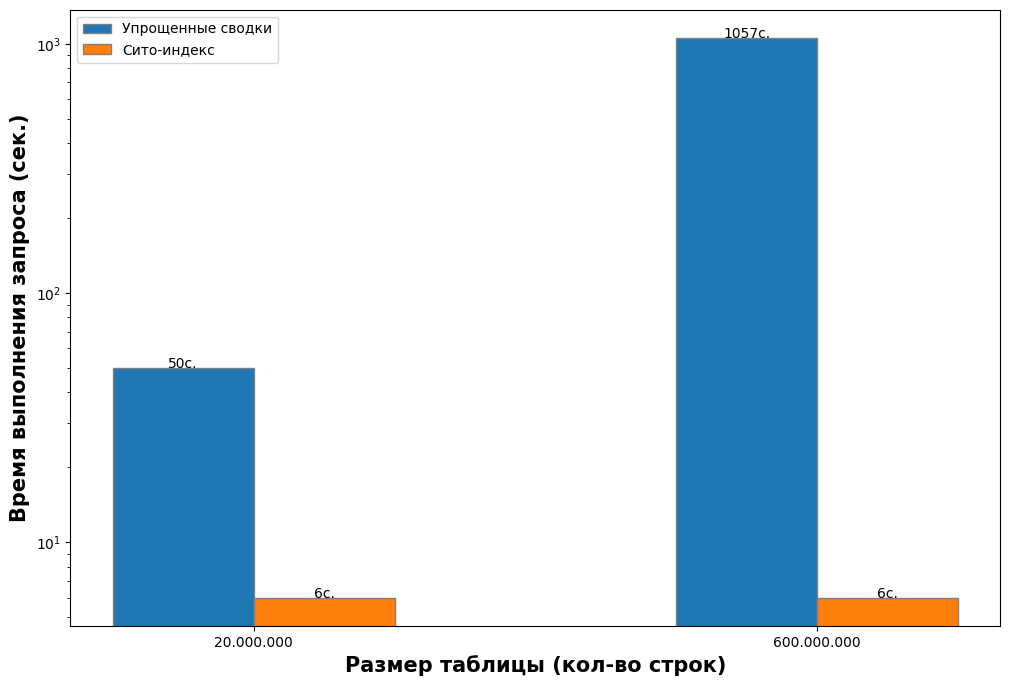
\includegraphics[scale=0.62]{1_point_query.png}
    \caption{\centering{Сравнение времени выполнения точечного запроса с использованием упрощенных сводок и Сито-индекса на двух таблицах разного размера}}
\end{figure}


\begin{figure}[p]
    \centering
    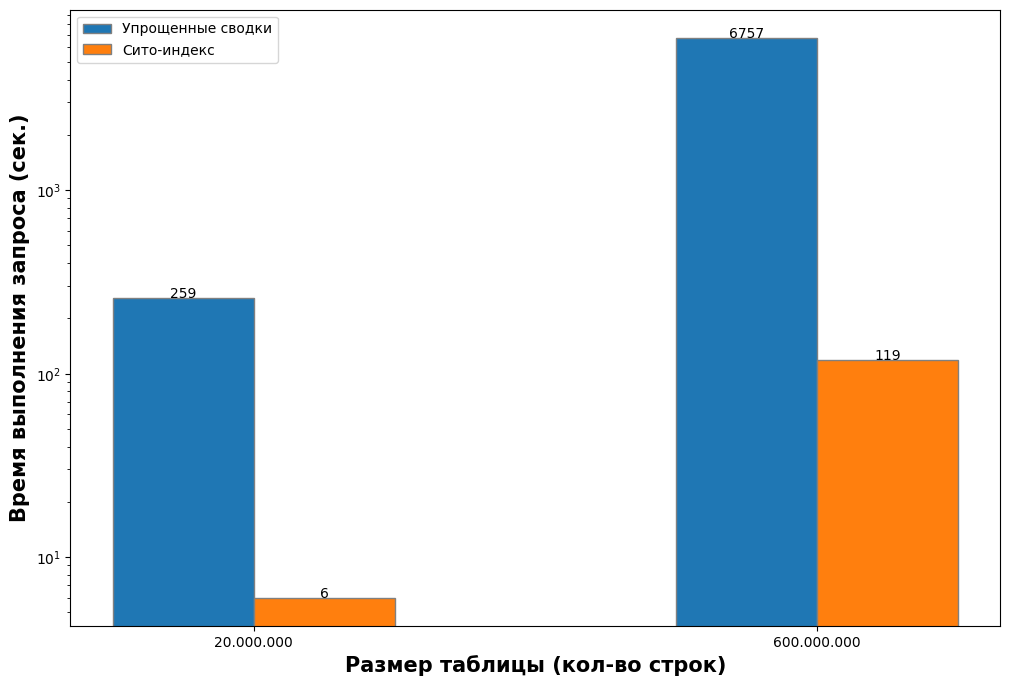
\includegraphics[scale=0.62]{2_range_query.png}
    \caption{\centering{Сравнение времени выполнения интервального запроса с использованием упрощенных сводок и Сито-индекса на двух таблицах разного размера}}
\end{figure}

\begin{figure}[p]
    \centering
    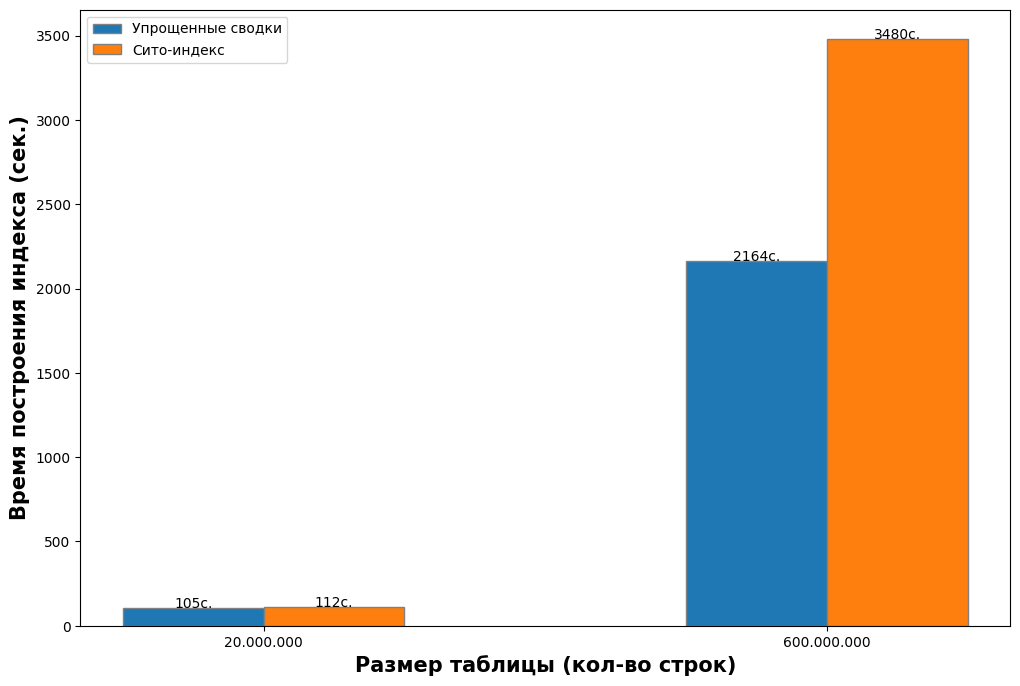
\includegraphics[scale=0.62]{3_build_time.png}
    \caption{\centering{Сравнение времени построения упрощенных сводок и Сито-индекса на двух таблицах разного размера}}
\end{figure}

\begin{figure}[h]
    \centering
    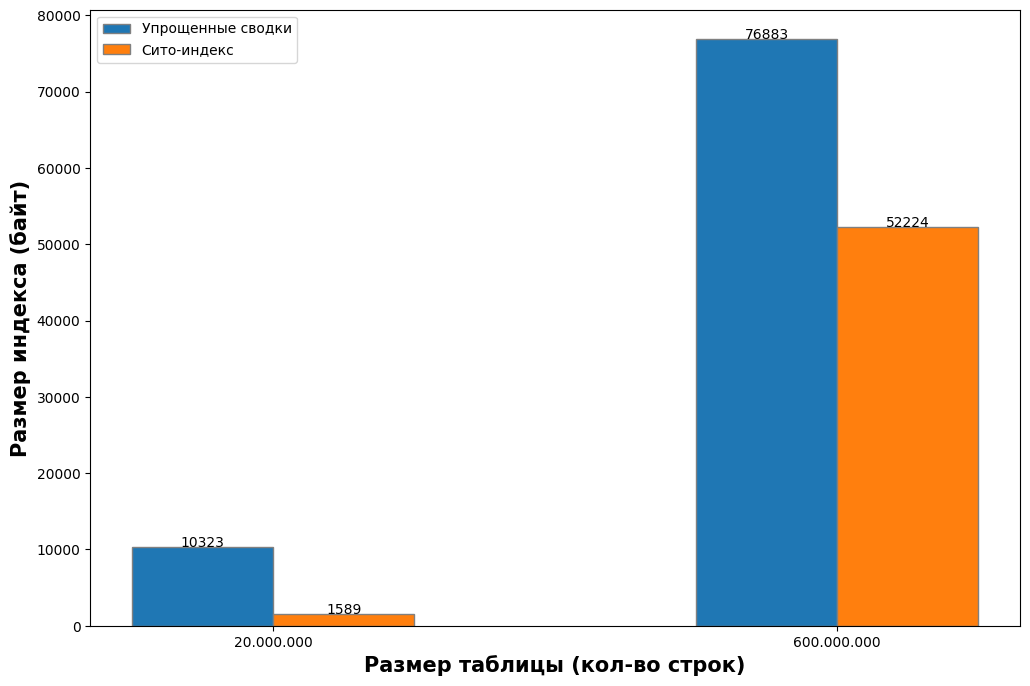
\includegraphics[scale=0.62]{4_index_size.png}
    \caption{\centering{Сравнение итогового размера упрощенных сводок и Сито-индекса на файловой системе для двух таблицах разного размера}}
\end{figure}

% \newpage
% \section*{Выводы}
% \addcontentsline{toc}{section}{Выводы}

% Следует подчеркнуть потенциал внедрения структуры данных Сито-индекс в современные платформы озер данных, такие как Apache Hudi, Iceberg и DeltaLake. Принципы работы с данными в них имеют много общего, что делает возможным применение Сито-индекса также и в других платформах.

% Особенностью Сито-индекса является его легковесность, позволяющая полностью загружать его в оперативную память. Это становится возможным благодаря тому, что размер индекса составляет всего десятые доли процента от общего объема данных. Такая эффективность открывает перспективы использования Сито-индекса не только в платформах озер данных, но и в SQL-движках, предназначенных для обработки больших данных, например, в Apache Presto.

% Индексация данных в рамках платформы Apache Hudi показала, что даже при работе с большими объемами данных (до 600 миллионов строк) возможно эффективное построение индекса, что подтверждает его применимость в условиях ограниченной памяти.
